% Created 2017-05-22 Mon 09:15
\documentclass{beamer}
\usepackage{fixltx2e}
\usepackage{graphicx}
\usepackage{longtable}
\usepackage{float}
\usepackage{wrapfig}
\usepackage{soul}
\usepackage{textcomp}
\usepackage{marvosym}
\usepackage{wasysym}
\usepackage{latexsym}
\usepackage{amssymb}
\usepackage{hyperref}
\tolerance=1000
\usepackage{etex}
\usepackage{amsmath}
\DeclareMathOperator*{\median}{median}
\usepackage{clrscode}
\usepackage{pstricks}
\usepackage{pgfplots}
\usepackage{tikz}
\usepackage[europeanresistors,americaninductors]{circuitikz}
\usepackage{colortbl}
\usepackage{yfonts}
\usetikzlibrary{shapes,arrows}
\usetikzlibrary{positioning}
\usetikzlibrary{arrows,shapes}
\usetikzlibrary{intersections}
\usetikzlibrary{calc,patterns,decorations.pathmorphing,decorations.markings}
\usepackage[BoldFont,SlantFont,CJKchecksingle]{xeCJK}
\setCJKmainfont[BoldFont=Evermore Hei]{Evermore Kai}
\setCJKmonofont{Evermore Kai}
\usepackage{pst-node}
\usepackage{pst-plot}
\psset{unit=5mm}
\usepackage{beamerarticle}
\mode<beamer>{\usetheme{Frankfurt}}
\mode<beamer>{\usecolortheme{dove}}
\mode<article>{\hypersetup{colorlinks=true,pdfborder={0 0 0}}}
\AtBeginSection[]{\begin{frame}<beamer>\frametitle{Topic}\tableofcontents[currentsection]\end{frame}}
\setbeamercovered{transparent}
\providecommand{\alert}[1]{\textbf{#1}}

\title{彩色图像处理}
\author{}
\date{}
\hypersetup{
  pdfkeywords={},
  pdfsubject={},
  pdfcreator={Emacs Org-mode version 7.9.3f}}

\begin{document}

\maketitle

\begin{frame}
\frametitle{Outline}
\setcounter{tocdepth}{3}
\tableofcontents
\end{frame}













\section{彩色基础}
\label{sec-1}
\begin{frame}
\frametitle{为什么要研究彩色图像处理?}
\label{sec-1-1}

\begin{itemize}
\item 符合人类视觉特点
\begin{itemize}
\item 人类可以辨别几千种颜色色调和亮度
\item 只能辨别几十种灰度层次
\end{itemize}
\item 特征描述
\begin{itemize}
\item 简化目标物的区分
\item 目标识别:根据目标的颜色特征
\end{itemize}
\end{itemize}
\end{frame}
\begin{frame}
\frametitle{研究领域}
\label{sec-1-2}

\begin{itemize}
\item 全彩色处理:全彩色传感器获取
\begin{itemize}
\item 彩色相机
\item 彩色扫描仪
\end{itemize}
\item 伪彩色处理: 对不同的灰度或灰度范围赋予不同的颜色
\end{itemize}
\end{frame}
\begin{frame}
\frametitle{颜色特性}
\label{sec-1-3}

描述彩色光的3个基本量:
\begin{itemize}
\item 辐射率:从光源流出能量的总量,用瓦特(W)度量
\item 光强:观察者从光源接收的能量总和
\item 亮度:主观描绘子
\end{itemize}
\end{frame}
\begin{frame}
\frametitle{颜色分解与合成}
\label{sec-1-4}

\begin{itemize}
\item 三原色 :  红色(Red)、绿色(Green)、蓝色(Blue)
\item 原色相加可产生二次色
\begin{itemize}
\item 深红色:红+蓝
\item 青色:绿+蓝
\item 黄色:红+绿
\end{itemize}
\end{itemize}
\end{frame}
\section{彩色模型}
\label{sec-2}
\begin{frame}
\frametitle{彩色空间}
\label{sec-2-1}

\begin{itemize}
\item RGB
\item CMY和CMYK
\item HSI
\item YIQ
\item YUV
\item YCbCr
\end{itemize}
\end{frame}
\begin{frame}
\frametitle{RGB}
\label{sec-2-2}

\begin{itemize}
\item CCD技术直接感知R,G,B三个分量
\item 是图像成像、显示、打印等设备的基础
\end{itemize}
\includegraphics[width=0.3\textwidth]{./image/light_r.png}
\includegraphics[width=0.3\textwidth]{./image/light_g.png}
\includegraphics[width=0.3\textwidth]{./image/light_b.png}
\end{frame}
\begin{frame}
\frametitle{RGB颜色空间}
\label{sec-2-3}

\includegraphics[width=0.5\textwidth]{./image/rgb_cube.png}
\includegraphics[width=0.5\textwidth]{./image/CIE1931xy_blank.png}
\end{frame}
\begin{frame}
\frametitle{CMY和CMYK彩色空间}
\label{sec-2-4}

\begin{itemize}
\item CMY(青、深红、黄)、CMYK (青、深红、黄、黑)
\item 运用在大多数在纸上沉积彩色颜料的设备,如彩色打印机和复印机
\item CMYK
\begin{itemize}
\item 打印中的主要颜色是黑色
\item 等量的CMY原色产生黑色,但不纯
\item 在CMY基础上,加入黑色,形成CMYK彩色空间
\end{itemize}
\end{itemize}
\end{frame}
\begin{frame}
\frametitle{HSI(色调、饱和度、亮度)}
\label{sec-2-5}

\begin{itemize}
\item 特点:
\begin{itemize}
\item I分量与图像的彩色信息无关
\item H和S分量与人感受颜色的方式是紧密相连的
\end{itemize}
\item 广泛用于计算机视觉、图像检索和视频检索
\begin{itemize}
\item 将亮度(I)与色调(H)和饱和度(S)分开
\item 避免颜色受到光照明暗(I)等条件的干扰
\item 可分析反映色彩本质的色调和饱和度
\end{itemize}
\end{itemize}
\end{frame}
\begin{frame}
\frametitle{HSI}
\label{sec-2-6}

\centering
\includegraphics[width=.9\linewidth]{./image/HSIColorModel.jpg}
\end{frame}
\begin{frame}
\frametitle{YIQ}
\label{sec-2-7}

\begin{itemize}
\item Y指亮度(Brightness),即灰度值
\item I和Q指色调,描述色彩及饱和度
\item 用于彩色电视广播,被北美的电视系统所采用(属于NTSC系统)
\item Y分量可提供黑白电视机的所有影像信息
\end{itemize}
\end{frame}
\begin{frame}
\frametitle{YUV}
\label{sec-2-8}

\begin{itemize}
\item Y指亮度,与YIQ的Y相同
\item U和V也指色调,不同于YIQ的I和Q
\item 用于彩色电视广播,被欧洲的电视系统所采用(属于PAL系统)
\item Y分量也可提供黑白电视机的所有影像信息
\end{itemize}
\end{frame}
\begin{frame}
\frametitle{YCbCr}
\label{sec-2-9}

\begin{itemize}
\item Y指亮度,与YIQ和YUV的Y相同
\item Cb和Cr由U和V调整得到
\item JPEG采用的彩色空间
\end{itemize}
\end{frame}
\section{颜色空间转换}
\label{sec-3}
\begin{frame}
\frametitle{颜色空间转换}
\label{sec-3-1}

\begin{itemize}
\item RGB $\leftrightarrow$   CMY
\item RGB $\leftrightarrow$  HSI
\item RGB $\leftrightarrow$  YIQ
\item RGB $\leftrightarrow$  YUV
\item RGB $\leftrightarrow$   YCbCr
\end{itemize}
\end{frame}
\begin{frame}
\frametitle{RGB-CMY}
\label{sec-3-2}


RGB和CMY值都归一化到  $[0,1]$

\[ \begin{bmatrix}
C \\
M\\
Y
\end{bmatrix}=
\begin{bmatrix}
1\\
1\\
1
\end{bmatrix}-
\begin{bmatrix}
R\\
G\\
B
\end{bmatrix} \]
\end{frame}
\begin{frame}
\frametitle{RGB $\to$ HSI}
\label{sec-3-3}

\begin{align*}
\theta &=\arccos\frac{\frac{1}{2}((R-G)+(R-B))}{((R-G)^2+(R-G)(G-B))^{\frac{1}{2}}}\\
H &=
\begin{cases}
\theta, \qquad B\leq G \\
360-\theta, \qquad B>G
\end{cases} \\
S &= 1 - \frac{3}{R+G+B}\min(R,G,B) \\
I &= \frac{1}{3}(R+G+B)
\end{align*}
\end{frame}
\begin{frame}
\frametitle{HSI $\to$ RGB}
\label{sec-3-4}

\begin{itemize}
\item $0^{\circ}\leq H<120^{\circ}$ 时
   \[ R = I\left(1+\frac{S\cos H}{\cos(60^{\circ}-H)}\right),B = I(1-S),G = 1-(R+B) \]
\item $120^{\circ}\leq H<240^{\circ}$ 时
   \begin{align*}
    &H =H-120^{\circ} \\
    &G = I\left(1+\frac{S\cos H}{\cos(60^{\circ}-H)}\right), R = I(1-S), B = 1-(R+G)
    \end{align*}
\item $240^{\circ}\leq H<360^{\circ}$ 时
   \begin{align*}
   &H =H-240^{\circ}\\ 
   &B = I\left(1+\frac{S\cos H}{\cos(60^{\circ}-H)}\right), G = I(1-S), R = 1-(B+G)
  \end{align*}
\end{itemize}
\end{frame}
\begin{frame}
\frametitle{RGB-YIQ}
\label{sec-3-5}

\begin{align*}
\begin{bmatrix}
Y\\
I\\
Q
\end{bmatrix}
&=
\begin{bmatrix}
 0.299 & 0.587 & 0.114 \\ 
 0.596 & -0.274 & -0.322 \\
 0.211 & -0.523 & 0.312 
\end{bmatrix}
\begin{bmatrix}
R\\
G\\
B\\
\end{bmatrix}\\
\begin{bmatrix}
R\\
G\\
B\\
\end{bmatrix}
&=
\begin{bmatrix}
 1  & 0.956 &  0.621 \\
 1  & -0.272 &  -0.647 \\
 1  & -1.106 &  1.703 
\end{bmatrix}
\begin{bmatrix}
Y\\
I\\
Q
\end{bmatrix}
\end{align*}
\end{frame}
\section{彩色图像处理}
\label{sec-4}
\begin{frame}
\frametitle{伪彩色图像处理}
\label{sec-4-1}


\begin{itemize}
\item 也叫假彩色图像处理
\item 根据一定的准则对灰度值赋以彩色的处理
\item 区分:伪彩色图像、真彩色图像、单色图像
\item 为什么需要伪彩色图像处理?
\begin{itemize}
\item 人类可以辨别上千种颜色和强度
\item 只能辨别二十几种灰度
\end{itemize}
\item 应用
\begin{itemize}
\item 为人们观察和解释图像中的灰度目标
\end{itemize}
\end{itemize}
\end{frame}
\begin{frame}
\frametitle{怎样进行伪彩色图像处理?}
\label{sec-4-2}

\begin{itemize}
\item 强度分层技术
\item 灰度级到彩色转换技术
\end{itemize}
\end{frame}
\begin{frame}
\frametitle{强度分层技术}
\label{sec-4-3}

\begin{itemize}
\item 令 $[0,L-1]$ 表示灰度级,使 $l_0$ 代表黑色 $(f(x,y)=0)$, $l_{L-1}$ 代表白色 ($f(x,y)=L-1$)。
\item 假设垂直于强度轴的 $P$ 个平面定义为量级 $l_1,l_2,\cdots,l_P$ 。$0<P<L-1$ , $P$ 个平面将灰度级分为 $P+1个$ 间隔, $V_1,V_2,\cdots,V_{P+1}$ ,
\item 则灰度级到彩色的赋值关系:
   \[ f(x,y)=c_k,  \qquad f(x,y)\in V_k \]
\item $c_k$ 是与强度间隔
\item $V_k$ 第 $K$ 级强度有关的颜色
\item $V_k$ 是由在 $l=k-1$ 和 $l=k$ 分割平面定义的
\end{itemize}
\end{frame}
\begin{frame}
\frametitle{灰度级到彩色的转换}
\label{sec-4-4}

\begin{itemize}
\item 对任何输入像素的灰度级执行3个独立变换
\item 3个变换结果分别送入彩色监视器的红、绿、蓝三个通道
\item 合成彩色图像
\end{itemize}
\end{frame}
\begin{frame}
\frametitle{伪彩色处理}
\label{sec-4-5}

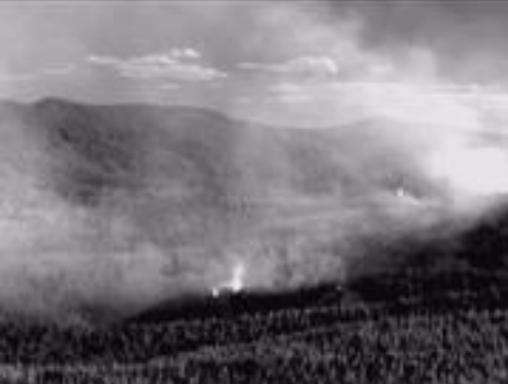
\includegraphics[width=0.3\textwidth]{./image/timg.jpeg}
\includegraphics[width=0.3\textwidth]{./image/rgblut.png}
\includegraphics[width=0.3\textwidth]{./image/timgcolor.png}
\end{frame}
\begin{frame}
\frametitle{全彩色图像处理}
\label{sec-4-6}

\begin{itemize}
\item 全彩色图像处理研究分为两大类:
\begin{itemize}
\item 分别处理每一分量图像,然后,合成彩色图像
\item 直接对彩色像素处理:3个颜色分量表示像素向量。
\end{itemize}
\end{itemize}
\end{frame}
\section{彩色变换}
\label{sec-5}
\begin{frame}
\frametitle{彩色变换函数}
\label{sec-5-1}


   \[ g(x,y)=T[f(x,y)] \]

\begin{itemize}
\item $f(x,y)$ 是彩色输入图像
\item $g(x,y)$ 是变换或处理过的彩色输出图像
\item $T$ 是在 $(x,y)$ 的空间邻域上对 $f(x,y)$ 的操作
\end{itemize}
\end{frame}
\begin{frame}[fragile]
\frametitle{亮度变换}
\label{sec-5-2}
\begin{block}{亮度变换示例}
\label{sec-5-2-1}

\includegraphics[width=0.3\textwidth]{./image/coffee.png}
\includegraphics[width=0.3\textwidth]{./image/coffeebright.png}
\includegraphics[width=0.3\textwidth]{./image/coffeedark.png}
\end{block}
\begin{block}{程序}
\label{sec-5-2-2}


\begin{verbatim}
from skimage import data,io
import  numpy as np
image=data.coffee()
brighter=np.uint8(image*0.5+255*0.5)
darker=np.uint8(image*0.5)
invert=255-image
\end{verbatim}
\end{block}
\end{frame}
\begin{frame}
\frametitle{补色}
\label{sec-5-3}

\includegraphics[width=0.45\textwidth]{./image/coffee.png}
\includegraphics[width=0.45\textwidth]{./image/coffeeinvert.png}
\end{frame}
\begin{frame}
\frametitle{彩色分层}
\label{sec-5-4}

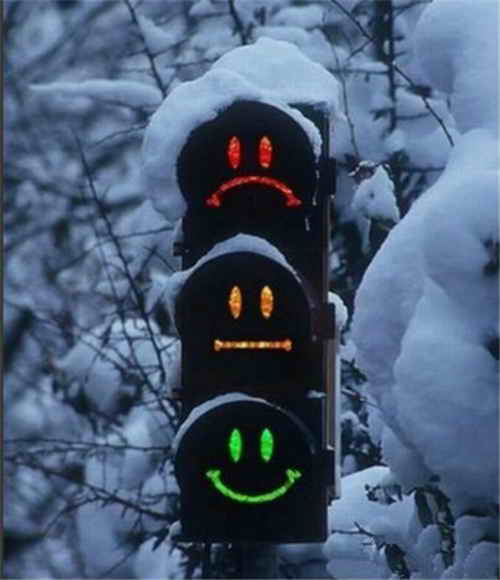
\includegraphics[width=0.25\textwidth]{./image/trafficlight.png}
\includegraphics[width=0.25\textwidth]{./image/lightred.png}
\includegraphics[width=0.25\textwidth]{./image/lightgreen.png}
\includegraphics[width=0.25\textwidth]{./image/lightyellow.png}
\end{frame}
\begin{frame}[fragile]
\frametitle{色调和彩色校正}
\label{sec-5-5}
\begin{block}{调整饱和度}
\label{sec-5-5-1}

\includegraphics[width=0.3\textwidth]{./image/astronaut.png}
\includegraphics[width=0.3\textwidth]{./image/astronautlight.png}
\includegraphics[width=0.3\textwidth]{./image/astronautdark.png}
\end{block}
\begin{block}{程序}
\label{sec-5-5-2}


\begin{verbatim}
image=data.astronaut()
h1=color.rgb2hsv(image)
h2=h1.copy()
h1[:,:,1]=h1[:,:,1]*0.5
h2[:,:,1]=h2[:,:,1]*0.5+0.5
\end{verbatim}
\end{block}
\end{frame}
\begin{frame}[fragile]
\frametitle{色调和彩色校正}
\label{sec-5-6}
\begin{block}{改变颜色分量}
\label{sec-5-6-1}

\includegraphics[width=0.3\textwidth]{./image/astronautred.png}
\includegraphics[width=0.3\textwidth]{./image/astronautyellow.png}
\includegraphics[width=0.3\textwidth]{./image/astronautblue.png}
\end{block}
\begin{block}{程序}
\label{sec-5-6-2}


\begin{verbatim}
imagered[:,:,0]=image[:,:,0]*127.0/255+128
imageyellow[:,:,0]=image[:,:,0]*127.0/255+128
imageyellow[:,:,1]=image[:,:,1]*127.0/255+128
imageblue[:,:,2]=image[:,:,2]*127.0/255+128
\end{verbatim}
\end{block}
\end{frame}
\begin{frame}
\frametitle{HSI颜色空间下的直方图均衡}
\label{sec-5-7}

\includegraphics[width=0.5\textwidth]{./image/astronaut.png}
\includegraphics[width=0.5\textwidth]{./image/astronautequal.png}
\end{frame}
\section{彩色图像平滑、锐化}
\label{sec-6}
\begin{frame}
\frametitle{彩色图像平滑}
\label{sec-6-1}

令 $S_{xy}$ 表示 $(x,y)$ 邻域的坐标集, ,在该邻域中RGB分量的平均值为

\begin{align*}
\bar c(x,y) &=\frac{1}{k}\sum_{(x,y)\in S_{xy}}c(x,y) \\
 c(x,y) &=
\begin{bmatrix}
R(x,y)\\
G(x,y)\\
B(x,y)
\end{bmatrix}
\end{align*}
\end{frame}
\begin{frame}
\frametitle{彩色图像平滑}
\label{sec-6-2}

\includegraphics[width=0.3\textwidth]{./image/astronautgaussian3.png}
\includegraphics[width=0.3\textwidth]{./image/astronautgaussian9.png}
\includegraphics[width=0.3\textwidth]{./image/astronautgaussian15.png}
\end{frame}
\begin{frame}
\frametitle{彩色图像锐化(拉普拉斯微分)}
\label{sec-6-3}

RGB彩色空间,分别计算每一分量图像的拉普拉斯变换
\begin{align*}
\nabla^2c(x,y) &=
\begin{bmatrix}
\nabla^2 R(x,y)\\
\nabla^2 G(x,y)\\
\nabla^2 B(x,y)
\end{bmatrix}\\
g(x,y) ={} & f(x,y)-\nabla^2 f(x,y) \\
 = {} & f(x,y)-(f(x+1,y)+f(x-1,y)+f(x,y+1)+f(x,y-1) \\
  & - 4f(x,y)) \\
={} & 5f(x,y)-(f(x+1,y)+f(x-1,y)+f(x,y+1)+f(x,y-1))
\end{align*}
\end{frame}
\begin{frame}
\frametitle{锐化示例(RGB分量锐化与HSV空间V分量锐化)}
\label{sec-6-4}

\includegraphics[width=0.3\textwidth]{./image/astronautgaussian3.png}
\includegraphics[width=0.3\textwidth]{./image/astronautsharprgb.png}
\includegraphics[width=0.3\textwidth]{./image/astronautsharphsv.png}
\end{frame}
\section{彩色分割}
\label{sec-7}
\begin{frame}
\frametitle{彩色分割}
\label{sec-7-1}

\begin{itemize}
\item RGB彩色空间——直接
\item HSI彩色空间分割——物理意义明确
\begin{itemize}
\item H色调图像方便描述彩色
\item S饱和度图像做模板分离感兴趣的特征区
\item I强度图像不携带彩色信息
\end{itemize}
\end{itemize}
\end{frame}
\begin{frame}
\frametitle{RGB彩色空间分割}
\label{sec-7-2}

令z代表RGB空间中的任意一点,a是分割颜色样本集的平均颜色向量
\begin{align*}
 D(z,a) &= ||z-a|| \\
&= \sqrt{(z_R-a_R)^2+(z_G-a_G)^2+(z_B-a_b)^2}
\end{align*}

\begin{itemize}
\item $D_0$ 是距离阈值
\item 如果 $D(z,a) \leq D_0$ , 则z和a相似
\item 如果 $D(z,a) > D_0$ , 则z和a不相似
\end{itemize}
\end{frame}
\begin{frame}
\frametitle{RGB颜色分割}
\label{sec-7-3}

\includegraphics[width=0.3\textwidth]{./image/astronautsegr.png}
\includegraphics[width=0.3\textwidth]{./image/astronautsegg.png}
\includegraphics[width=0.3\textwidth]{./image/astronautsegb.png}
\end{frame}
\begin{frame}
\frametitle{彩色边缘检测}
\label{sec-7-4}

\begin{align*}
\vec{u} &= \frac{\partial R}{\partial x}\vec{r}+\frac{\partial G}{\partial x}\vec{g}+\frac{\partial B}{\partial x}\vec{b} \\
\vec{v} &= \frac{\partial R}{\partial y}\vec{r}+\frac{\partial G}{\partial y}\vec{g}+\frac{\partial B}{\partial y}\vec{b} \\
g_{xx} &= \vec{u}\cdot \vec{u}=\left(\frac{\partial R}{\partial x}\right)^2+\left(\frac{\partial G}{\partial x}\right)^2+\left(\frac{\partial B}{\partial x}\right)^2\\
g_{yy} &= \vec{v}\cdot \vec{v}=\left(\frac{\partial R}{\partial y}\right)^2+\left(\frac{\partial G}{\partial y}\right)^2+\left(\frac{\partial B}{\partial y}\right)^2\\
g_{xy} &= \vec{u}\cdot \vec{v}= \frac{\partial R}{\partial x}\frac{\partial R}{\partial y}+\frac{\partial G}{\partial x}\frac{\partial G}{\partial y}+\frac{\partial B}{\partial x}\frac{\partial B}{\partial y}\\
\theta &= \frac{1}{2}\arctan\left(\frac{2g_{xy}}{g_{xx}-g_{yy}}\right)\\
F(\theta) &=\left(\frac{1}{2}((g_{xx}+g_{yy})+(g_{xx}-g_{yy})\cos 2\theta +2g_{xy}\sin 2\theta)\right)^{\frac{1}{2}}
\end{align*}
\end{frame}
\begin{frame}
\frametitle{彩色边缘检测}
\label{sec-7-5}

\includegraphics[width=0.3\textwidth]{./image/astronautedger.png}
\includegraphics[width=0.3\textwidth]{./image/astronautedgeg.png}
\includegraphics[width=0.3\textwidth]{./image/astronautedgeb.png}
\end{frame}
\section{彩色图像的噪声}
\label{sec-8}
\begin{frame}
\frametitle{彩色图像的噪声}
\label{sec-8-1}

\includegraphics[width=0.5\textwidth]{./image/astronautnoiseg.png}
\includegraphics[width=0.5\textwidth]{./image/astronautnoisei.png}
\end{frame}
\begin{frame}
\frametitle{RGB分量}
\label{sec-8-2}

\includegraphics[width=0.25\textwidth]{./image/astronautnoiseg.png}
\includegraphics[width=0.25\textwidth]{./image/astronautnoisegr.png}
\includegraphics[width=0.25\textwidth]{./image/astronautnoisegg.png}
\includegraphics[width=0.25\textwidth]{./image/astronautnoisegb.png}

\includegraphics[width=0.25\textwidth]{./image/astronautnoisei.png}
\includegraphics[width=0.25\textwidth]{./image/astronautnoiseir.png}
\includegraphics[width=0.25\textwidth]{./image/astronautnoiseig.png}
\includegraphics[width=0.25\textwidth]{./image/astronautnoiseib.png}
\end{frame}
\begin{frame}
\frametitle{HSV分量}
\label{sec-8-3}

\includegraphics[width=0.25\textwidth]{./image/astronautnoiseg.png}
\includegraphics[width=0.25\textwidth]{./image/astronautnoisegh.png}
\includegraphics[width=0.25\textwidth]{./image/astronautnoisegs.png}
\includegraphics[width=0.25\textwidth]{./image/astronautnoisegv.png}

\includegraphics[width=0.25\textwidth]{./image/astronautnoisei.png}
\includegraphics[width=0.25\textwidth]{./image/astronautnoiseih.png}
\includegraphics[width=0.25\textwidth]{./image/astronautnoiseis.png}
\includegraphics[width=0.25\textwidth]{./image/astronautnoiseiv.png}
\end{frame}

\end{document}
